%\documentclass[twocolumn, aps, superscriptaddress]{revtex4}
%\documentclass[reprint, prl, aps, showpacs]{revtex4-1}
\documentclass[preprint, aps, showpacs]{revtex4-1}

\usepackage{graphicx}
\usepackage{amsmath,amssymb}
%\usepackage[usenames,dvipsnames]{color}
%\usepackage[colorlinks=true, citecolor=blue, linkcolor=WildStrawberry]{hyperref}
%\usepackage[citecolor=blue]{hyperref}
%\usepackage[justification=centerfirst]{caption}
\usepackage{epstopdf}

%\usepackage[latin1]{inputenc}
\usepackage{tikz}
\usetikzlibrary{shapes,arrows}

\newcommand{\braket}[2]{\left\langle#1\, |\,#2\,\right\rangle}  %  < #1 | #2 >
\newcommand{\expec}[1]{\langle#1\rangle}  %  < #1 >
\newcommand{\drm}{{\rm d}}
\newcommand{\irm}{{\rm i}}
\newcommand{\beq}{\begin{equation}}
\newcommand{\eeq}{\end{equation}}
\newcommand{\bdm}{\begin{displaymath}}
\newcommand{\edm}{\end{displaymath}}
\newcommand{\T}[1]{\tilde{#1}}
\newcommand{\wT}[1]{\widetilde{#1}}
\newcommand{\Cdot}{\!\cdot\!}
\newcommand{\SNR}{\textnormal{SNR}}
\newcommand{\rednote}[1]{{\color{red} (#1)}}
\newcommand{\fixme}[1]{\textcolor{green}{\textbf{\textit{{#1}}}}}

\DeclareFontFamily{OT1}{pzc}{}
\DeclareFontShape{OT1}{pzc}{m}{it}{<-> s * [1.10] pzcmi7t}{}
\DeclareMathAlphabet{\mathpzc}{OT1}{pzc}{m}{it}

\def\dblone{\hbox{$1\hskip -1.2pt\vrule depth 0pt height 1.6ex width 0.7pt \vrule depth 0pt height 0.3pt width 0.12em$}}

\graphicspath{{./plots/}}
\begin{document}

\title{Prediction of surface wave velocities with historical seismic data}

\author{Michael Coughlin}
\affiliation{Division of Physics, Math, and Astronomy, California Institute of Technology, Pasadena, CA 91125, USA}

\author{Nicolas Arnaud}
\affiliation{LAL, Univ. Paris-Sud, CNRS/IN2P3, Universit\'e Paris-Saclay, F-91898 Orsay, France}
\affiliation{European Gravitational Observatory (EGO), I-56021 Cascina, Pisa, Italy}

\author{David Barker}
\affiliation{LIGO Hanford Observatory, Richland, WA 99352, USA}

\author{Sebastien Biscans}
\affiliation{LIGO Laboratory, Massachusetts Institute of Technology, Cambridge, MA 02138, USA}

\author{Christopher Buchanan}
\affiliation{Department of Physics and Astronomy, Louisiana State University, Baton Rouge, LA 70803-4001, USA}

\author{Eric Coughlin}
\affiliation{Department of Computer Science, Luther College, 700 College Dr, Decorah, IA 52101, USA}

\author{Fred Donovan}
\affiliation{LIGO Laboratory, Massachusetts Institute of Technology, Cambridge, MA 02138, USA}

\author{Paul Earle}
\affiliation{U.S. Geological Survey, Golden, CO 80401, USA}

\author{Jeremy Fee}
\affiliation{United States Geological Survey, Golden, CO 80401, USA}

\author{Irene Fiori}
\affiliation{European Gravitational Observatory (EGO), I-56021 Cascina, Pisa, Italy}

\author{Hunter Gabbard}
\affiliation{Albert-Einstein-Institut, Max-Planck-Institut f{\"u}r Gravitationsphysik, D-30167 Hannover, Germany}

\author{Michelle Guy}
\affiliation{United States Geological Survey, Golden, CO 80401, USA}

\author{Jan Harms}
\affiliation{INFN, Sezione di Firenze, Sesto Fiorentino, 50019, Italy\\
Universit\`a degli Studi di Urbino ``Carlo Bo'', I-61029 Urbino, Italy}

\author{Nikhil Mukund}
\affiliation{Inter-University Centre for Astronomy and Astrophysics (IUCAA), Post Bag 4, Ganeshkhind,  Pune 411 007, India}

\author{Matthew Perry}
\affiliation{Planetary Science Institute, Lakewood, CO 80401, USA}

\author{Hugh Radkins}
\affiliation{LIGO Hanford Observatory, Richland, WA 99352, USA}

\author{Bas Swinkels}
\affiliation{European Gravitational Observatory (EGO), I-56021 Cascina, Pisa, Italy}

\author{Keith Thorne}
\affiliation{LIGO Livingston Observatory, Livingston, LA 70754, USA}

\author{Jim Warner}
\affiliation{LIGO Hanford Observatory, Richland, WA 99352, USA}

\maketitle

\textbf{Earthquake early warning (EEW) is a burgeoning field dedicated to the rapid detection and characterization of earthquakes as well as the dissemination of that information to people and infrastructure in their path \cite{Al2012,KuAl2013a,KuAl2013b,KuHe2014,CoLa2009a,CoLa2009b,BoAl2014,HoKa2008,HoEA2011c,StAl2016}.
As these systems minimize the time required to calculate the source parameters of earthquakes (i.e. their location and magnitude), it becomes important to predict the ground motion that the earthquakes will cause as a function of location and distance with high accuracy.
In this analysis, we leverage the power of machine learning algorithms to improve both the ground velocity predictions as well as the lockloss predictions of \emph{Seismon}. We demonstrate an improvement from a factor of 5 to a factor of 3 in scatter of the error in the predicted ground velocity.
The idea of the analysis is to compare historical ground velocity measurements 
to predictions made using a machine learning algorithm. 
To access the accuracy and utility of our approach, we compare the estimates based only on rapid magnitude and location estimates to the amplitudes observed.
We find agreement within a factor of 3 by this metric.
Further, we compare measurements that include the less timely earthquake slip inversion and CMT information to the original amplitudes observed, resulting in a factor of 2 agreement.}

With the advent of gravitational-wave astronomy, it is essential to maximize the duty cycle of second generation gravitational-wave detectors such as the Laser Interferometer Gravitational-wave Observatory (LIGO) \cite{aligo}, Virgo \cite{avirgo}, and GEO600 \cite{Gr2010} detectors.
Any increase in duty cycle increases the sensitivity of gravitational-wave searches, including the observations of binary black hole mergers \cite{AbEA2016a,AbEA2016e}.
One source of ground motion that destabilizes the detectors are earthquakes
\cite{CoSt2015,CoEa2017}, despite seismic isolation systems designed to minimize such effects \cite{AbAd2002,StAb2009,MaLa2015}.

Many seismic and geodetic (GPS) sensor arrays exist that are producing rapid earthquake information products, from magnitude and location estimates to regional centroid moment tensors (CMTs) and advanced slip inversions.
With wide-ranging public warning systems in Mexico and Japan and smaller-scale systems in many other countries, warnings from seconds to minutes are now available to reduce the impact of earthquakes on society \cite{StAl2016}.
The short warning times arise out of the physical processes that drive the earthquake rupture, where warning is given by seismometers measuring P-waves ($\approx$\,8\,km/s) and S-waves ($\approx$\,4\,km/s).

The main goal of EEW methods is generating reliable relations (sometimes called source-scaling laws) between and earthquake source parameters and ground motion metrics. Examples in the time domain include peak ground acceleration, effective peak ground acceleration, peak ground velocity, and peak
ground displacement, while in the frequency domain, spectral accelerations, velocities, and displacements as well as predominant periods \cite{Do2003}. These source-scaling laws are applied to early portions of seismograms to make predictions about the magnitude for EEW \cite{AlGa2009}, important for hypocenter and magnitude computations in tsunamis \cite{MeCr2015}, hazard computations in engineering seismology \cite{PaMu2012}, and computation of the elastic response spectrum \cite{Ch2007}.

Early estimates of magnitudes tend to underestimate the energy released due to the non-instantaneous pattern of slip.
\cite{MeCr2015} showed that real-time GPS waveforms can rapidly determine the magnitude within the first minute of rupture and in many cases before rupture is complete.
real-time GPS seismic waveforms can be used to rapidly determine magnitude, typically within the first minute of rupture initiation and in many cases before the rupture is complete. 
For this reason, the early estimates of the ground velocity amplitudes are not as accurate as later values. 
The effects of these errors are particularly pronounced for larger earthquakes, where the estimates of the fault lengths become more important.
Thus, these larger earthquakes tend to have their amplitudes underpredicted.
The loss of performance that results from use of the rapid estimates is acceptable to use as rapid warnings.

In previous work \cite{CoEa2017}, Coughlin et al. used advances in early earthquake warning to develop a low-latency earthquake early warning client named \emph{Seismon}, which uses a real-time event messaging system of the U.S. Geological Survey (USGS) to mitigate the effects of teleseismic events on ground-based gravitational-wave detectors. 
Using information about the earthquake source characteristics such as time, location, depth, and magnitude, predictions as to the arrival time and ground velocity induced by the earthquakes were predicted.
We showed that about 90\% of events had a measured ground velocity within a factor of 5 of the predicted value.

Machine learning has recently become an important aspect of EEW and machine learning algorithms in general.
The \emph{MyShake} EEW system uses artificial neural networks to differentiate earthquake and human motions, with 98\% of earthquake records within 10\,km correctly identified, and only 7\% of people-induced transients appearing to be earthquakes to the algorithm  \cite{KoAl2016}.

\begin{figure*}[t]
\hspace*{-0.5cm}
 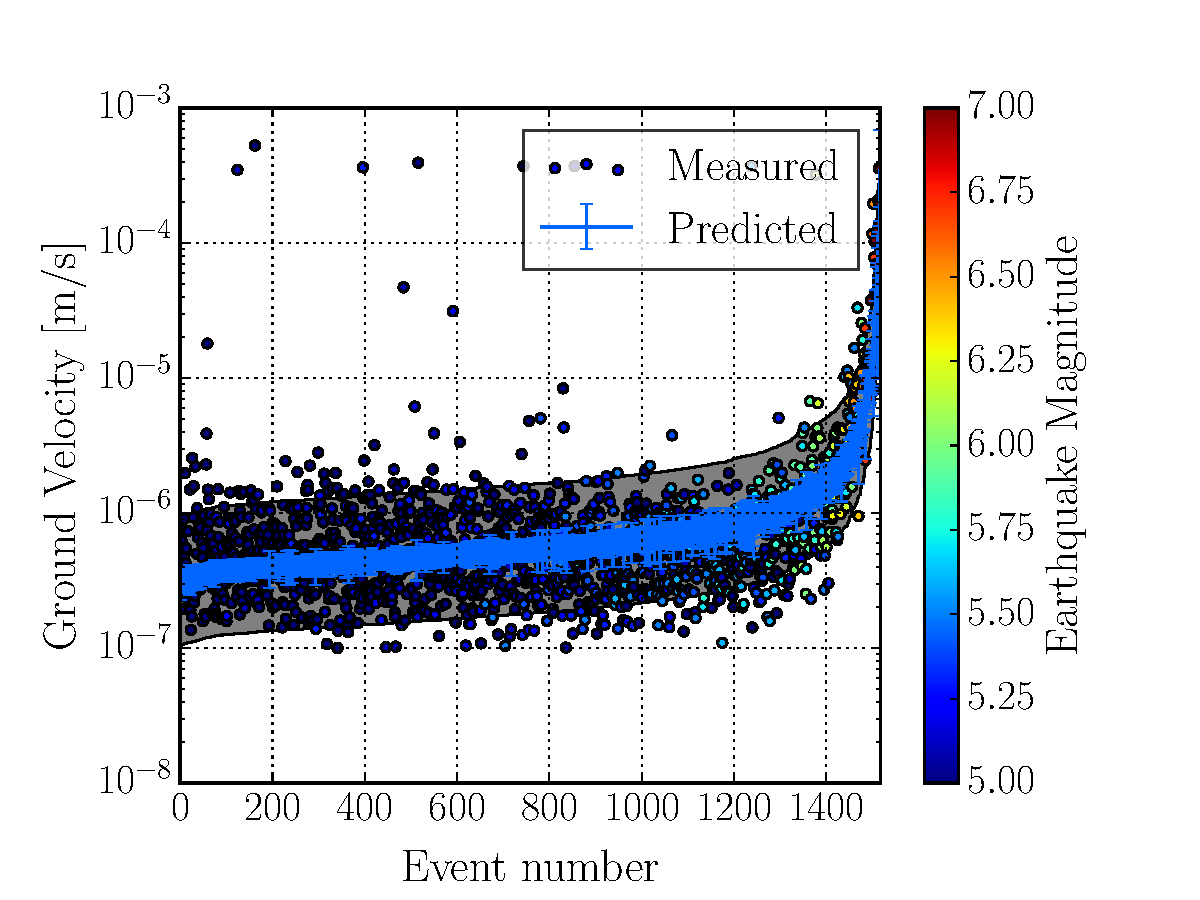
\includegraphics[width=3.5in,trim = 2.5cm 1.5cm 2.5cm 1.5cm, clip=true]{prediction_H1O1O2_GPR.pdf}
 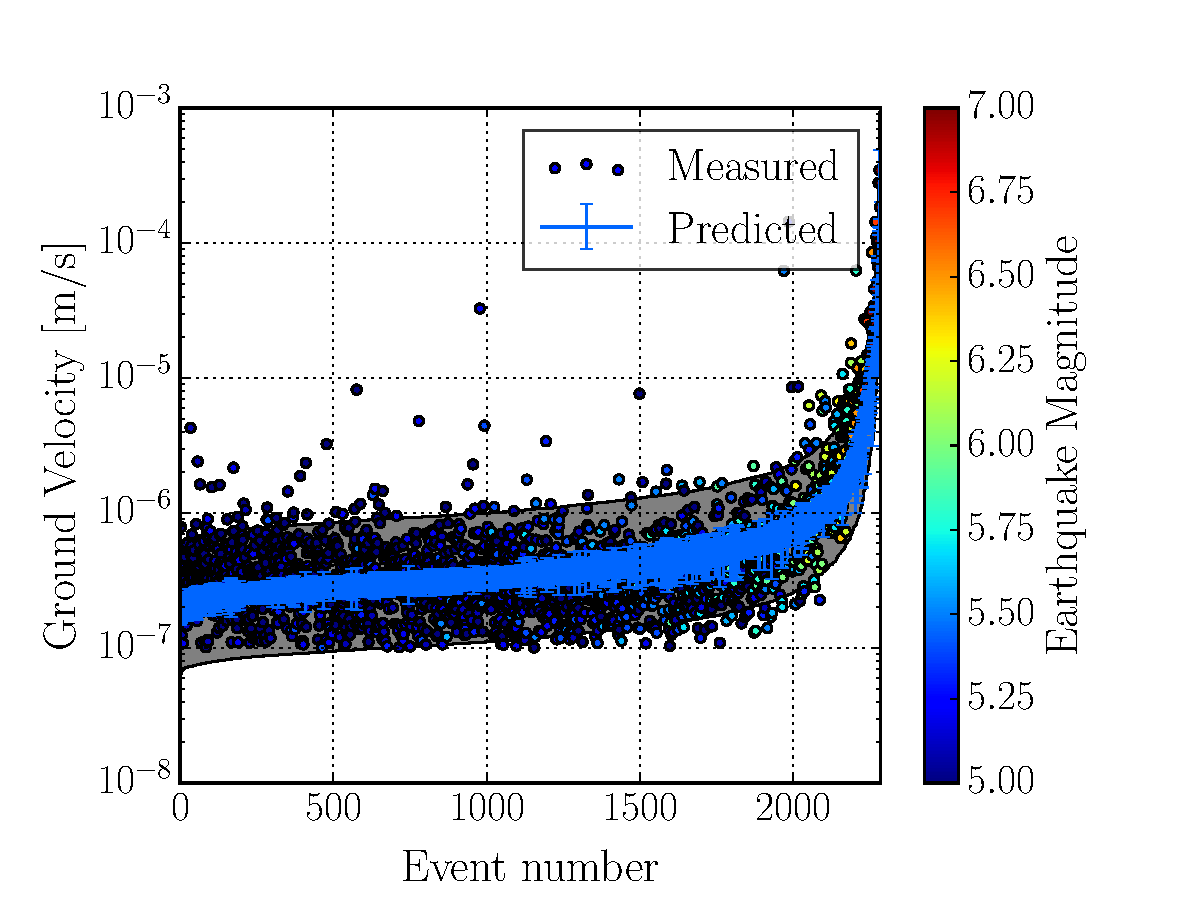
\includegraphics[width=3.5in,trim = 2.5cm 1.5cm 2.5cm 1.5cm, clip=true]{prediction_L1O1O2_GPR.pdf}
 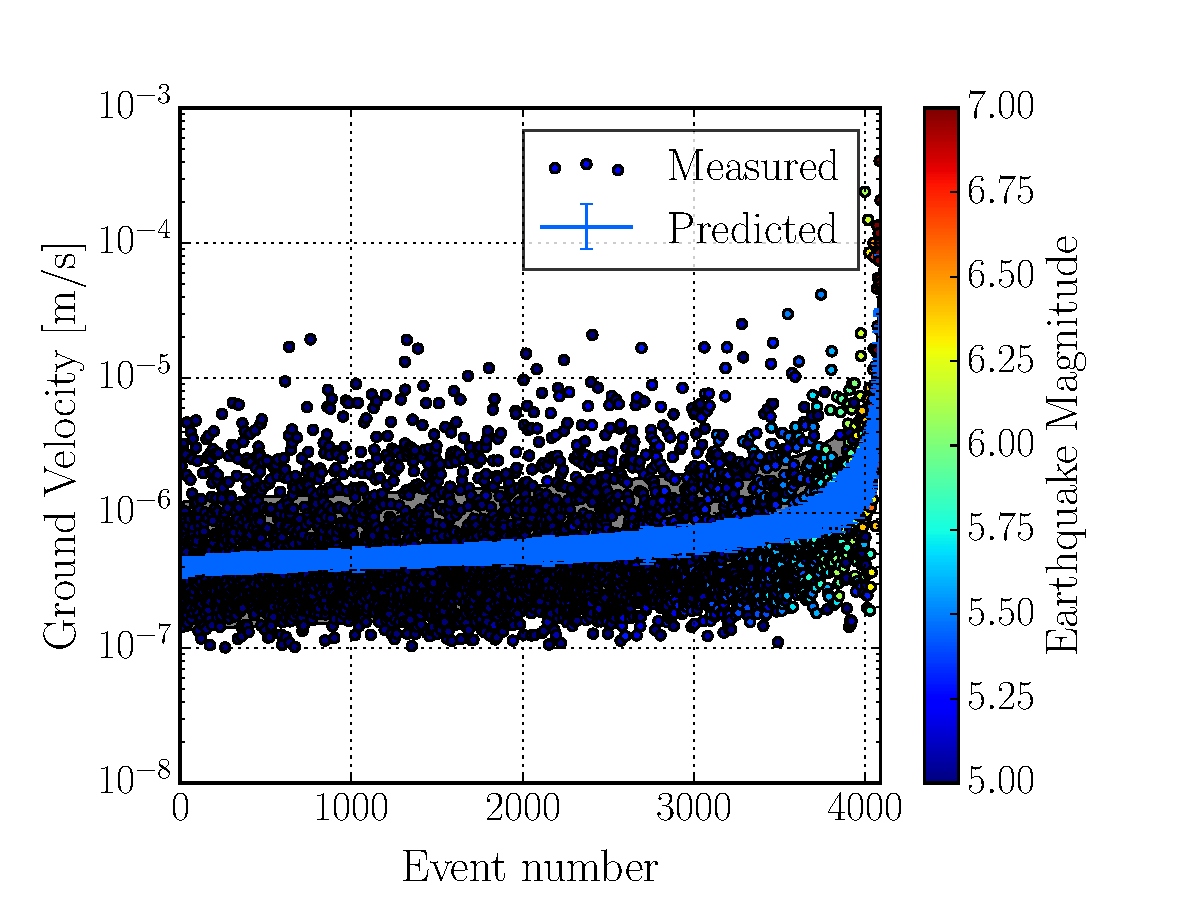
\includegraphics[width=3.5in,trim = 2.5cm 1.5cm 2.5cm 1.5cm, clip=true]{prediction_V1O1O2_GPR.pdf}
 \caption{Fit of peak velocities seen during O1-O2 at the interferometers (LHO, LLO, and Virgo) using Gaussian Process Regression. The events have been ordered by their measured peak ground velocity (in blue) and gray error bar corresponds to a factor of 3 within the predicted value. About 90\% of events are within a factor of 3 of the predicted value.}
 \label{fig:regression}
\end{figure*}

One of the key aspects of \emph{Seismon} is the ground velocity predictions, $\rm Rf_{amp}$, for each site. These predictions have two purposes. 
First of all, they provide a meaningful metric which on-site-staff at the detectors can use to plan the response to the incoming earthquake. 
The predictions also serve as inputs to the algorithms which make lockloss predictions, which we will describe in the following.

In the initial version of the algorithm \cite{CoEa2017}, we used an empirical fit to an equation derived to account for physical effects. This equation succeeded in predicting peak ground velocity such that 90\% of events had a measured ground velocity within a factor of 5 of the predicted value.
There were a few downsides to this empirical fit.
First of all, while it was derived with physical effects in mind, it was predominantly an empirical construction.
It was also found that the parameters in the model were quite degenerate, which meant that parameters derived to be physically meaningful quantities showed significant differences from site to site which were unlikely to actually be very different.
Finally, to be useful to the detectors, there is a goal of a factor of 2 in error, which is much smaller than the factor of 5 scatter seen.

We now depend on a machine learning algorithm to make the ground velocity predictions. In particular, we use the scikit-learn implementation of Gaussian Process Regression (GPR) to make the predictions.
The inputs to the algorithm are the earthquake magnitude, latitude, longitude, distance, depth, and azimuth. 
The target output is the measured ground velocity.
This improves on the equation in a few ways.
First of all, the algorithm leverages the power of machine learning algorithms, which is not reliant on a functional form.
Second, it trivially includes more parameters, such as latitude, longitude, and earthquake azimuth relative to the detector.

\begin{figure*}[t]
\hspace*{-0.5cm}
 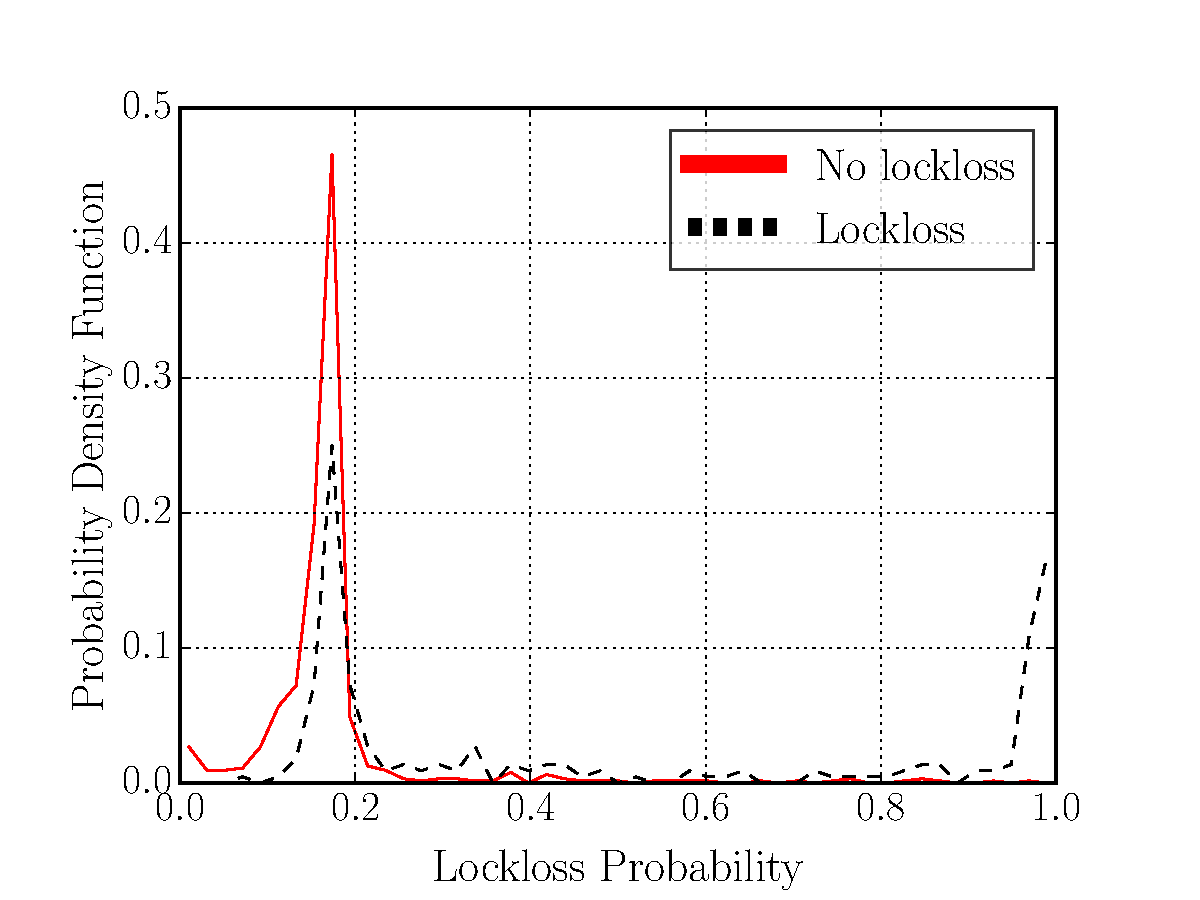
\includegraphics[width=3.5in,trim = 2.5cm 1.5cm 2.5cm 1.5cm, clip=true]{lockloss_histogram_H1O1O2_GPR.pdf}
 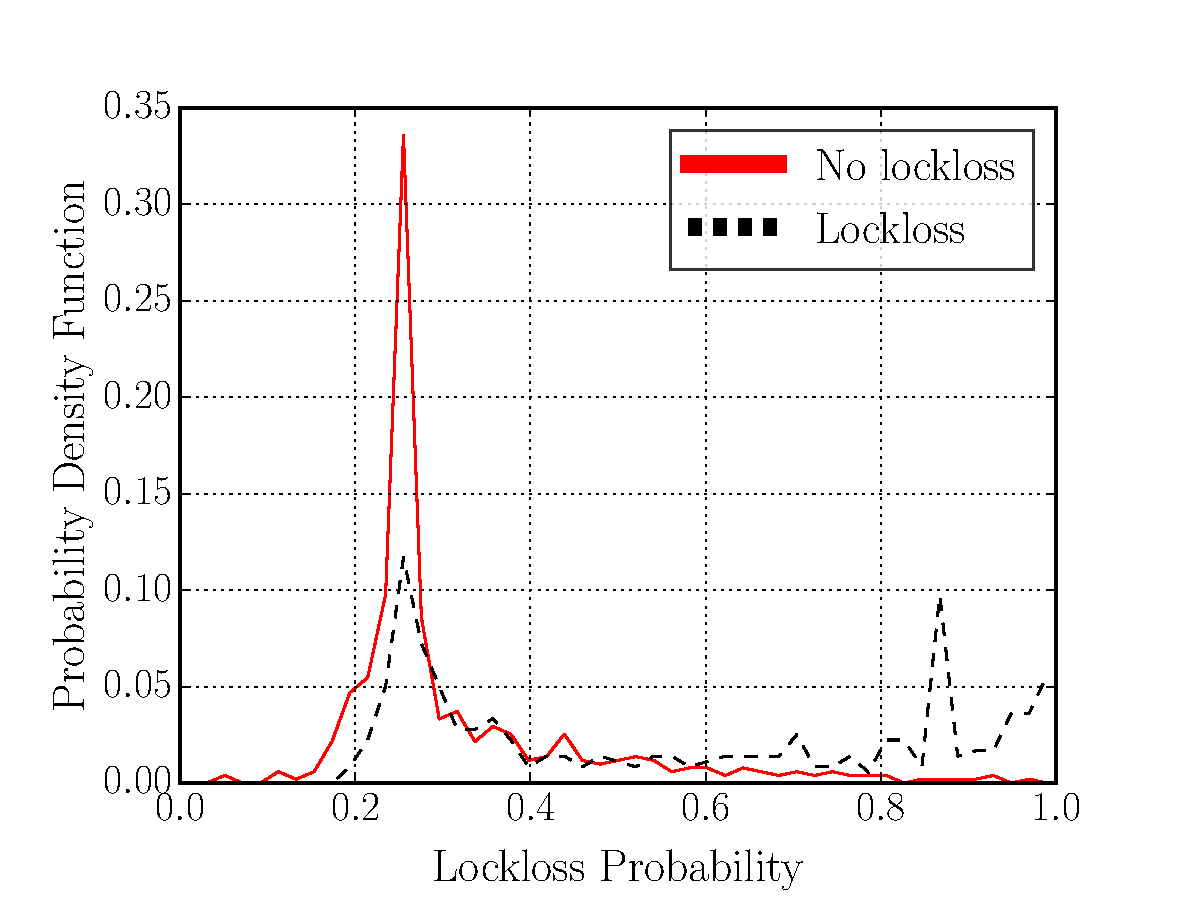
\includegraphics[width=3.5in,trim = 2.5cm 1.5cm 2.5cm 1.5cm, clip=true]{lockloss_histogram_L1O1O2_GPR.pdf}
 \caption{Histogram of lockloss probabilities predicted in O1-O2 at the interferometers (LHO and LLO) using Support Vector Machines.}
 \label{fig:lockloss}
\end{figure*}

It is useful to determine which earthquakes cause the loss of data and which will not affect the detector in a significant way.
In addition to the parameters that go into the ground velocity prediction model, we also use the prediction for the ground velocity to include when predicting the outcome of the interferometer lock status.
In previous work \cite{CoEa2017}, we found comparable performance among machine learning algorithms, and for this work use Support Vector Machines \cite{Burges_SVM}.
Figure~\ref{fig:lockloss} shows the distribution of the lockloss probabilities for O1 and O2 for both LHO and LLO. 

\textbf{Acknowledgments.}
MC was supported by the David and Ellen Lee Postdoctoral Fellowship at the California Institute of Technology.
NM acknowledges Council for Scientific and Industrial Research (CSIR), India, for providing financial support as Senior Research Fellow.  
LIGO was constructed by the California Institute of Technology and Massachusetts Institute of Technology with funding from the National Science Foundation and operates under cooperative agreement PHY-0757058.
This paper has been assigned LIGO document number LIGO-?.

%\raggedright
\bibliographystyle{unsrt}
\bibliography{references}

\textbf{Methods.}

\textbf{Gravitational-wave detectors.}

\textbf{Sources of seismic data.}


\textbf{Ground velocity predictions.}


\end{document} 
